Analizzando le concentrazioni misurate dalle stazioni di monitoraggio della qualità dell'aria e confrontandole con le misure degli anni precedenti, possiamo verificare se le riduzioni di emissioni (fig.\ref{fig:riduzioneemissioni}) abbiano determinato effetti sulla qualità dell'aria, e di quale entità. 

Gli andamenti delle mediane giornaliere regionali di benzene C\textsubscript{6}H\textsubscript{6}, biossido di azoto NO\textsubscript{2}, ozono O\textsubscript{3}, polveri sottili PM10 e PM2.5 (fig.\ref{fig:andaminq}), mostrano alcuni scostamenti del 2020 rispetto agli anni precedenti.

Il \textbf{benzene} ha generalmente concentrazioni più basse rispetto agli anni precedenti (fig.\ref{fig:andaminq}, primo pannello), ma poiché questa tendenza è già evidente prima del \textit{lockdown} e della chiusura delle scuole, è da attribuirsi ad una diminuzione delle emissioni che prescinde dalle azioni di contenimento. Tale tendenza si nota anche nell'analisi dei giorni tipo di alcune stazioni di monitoraggio, per esempio CAI (Udine, fig.\ref{fig:giornibenzene}). Inoltre, le stazioni industriali di Trieste (PIT e PON, fig.\ref{fig:giornibenzene}) non hanno registrato i picchi osservati negli anni scorsi, ascrivibili alle emissioni dell'area a caldo del polo siderurgico, ormai inattiva.

Il \textbf{biossido di azoto}, NO\textsubscript{2}, ha concentrazioni in linea con gli anni precedenti nelle prime settimane di febbraio (fig.\ref{fig:andaminq}, secondo pannello). Il calo progressivo che si osserva nei giorni 27 febbraio -- 7 marzo potrebbe essere determinato sia dalla chiusura delle scuole sia dalle condizioni meteo favorevoli alla dispersione (cfr.fig.\ref{fig:RSV}). Invece l'ulteriore calo nel periodo successivo, seppur accompagnato da fluttuazioni coerenti con le condizioni meteo, è da attribuire agli effetti del \textit{lockdown}. Infatti esso interessa tutta la regione (fig.\ref{fig:giornino2}, terza e quarta colonna) e corrisponde a un netto smorzamento dei picchi corrispondenti alle ore di punta nel traffico stradale, la mattina e la sera.

L'\textbf{ozono}, inquinante secondario di origine fotochimica, non risente in maniera evidente degli effetti del \textit{lockdown}. Le concentrazioni di aprile, più alte degli anni precedenti (fig.\ref{fig:andaminq}, terzo pannello), sono da attribuirsi alle temperature particolarmente miti di quelle settimane. I giorni medi conservano l'andamento tipico (fig.\ref{fig:giornio3}).

Le polveri \textbf{PM10} mostrano un vistoso picco di concentrazioni corrispondenti al trasporto a grande scala di polveri di origine desertica che ha interessato il Friuli Venezia Giulia nei giorni 27-29 marzo (fig.\ref{fig:andaminq}, quarto pannello). Il picco è meno marcato per le polveri più sottili \textbf{PM2.5} (fig.\ref{fig:andaminq}, quinto pannello), segno che le polveri desertiche avevano una granulometria grossolana. Al di là di questo fattore confondente, non si notano particolari scostamenti rispetto agli anni precedenti, neppure nei giorni tipo (fig.\ref{fig:giornipm10}). Si rimanda perciò all'analisi sulla granulometria delle polveri (pag.\ref{cap:cef} e sgg.).


\begin{figure}
    \centering
    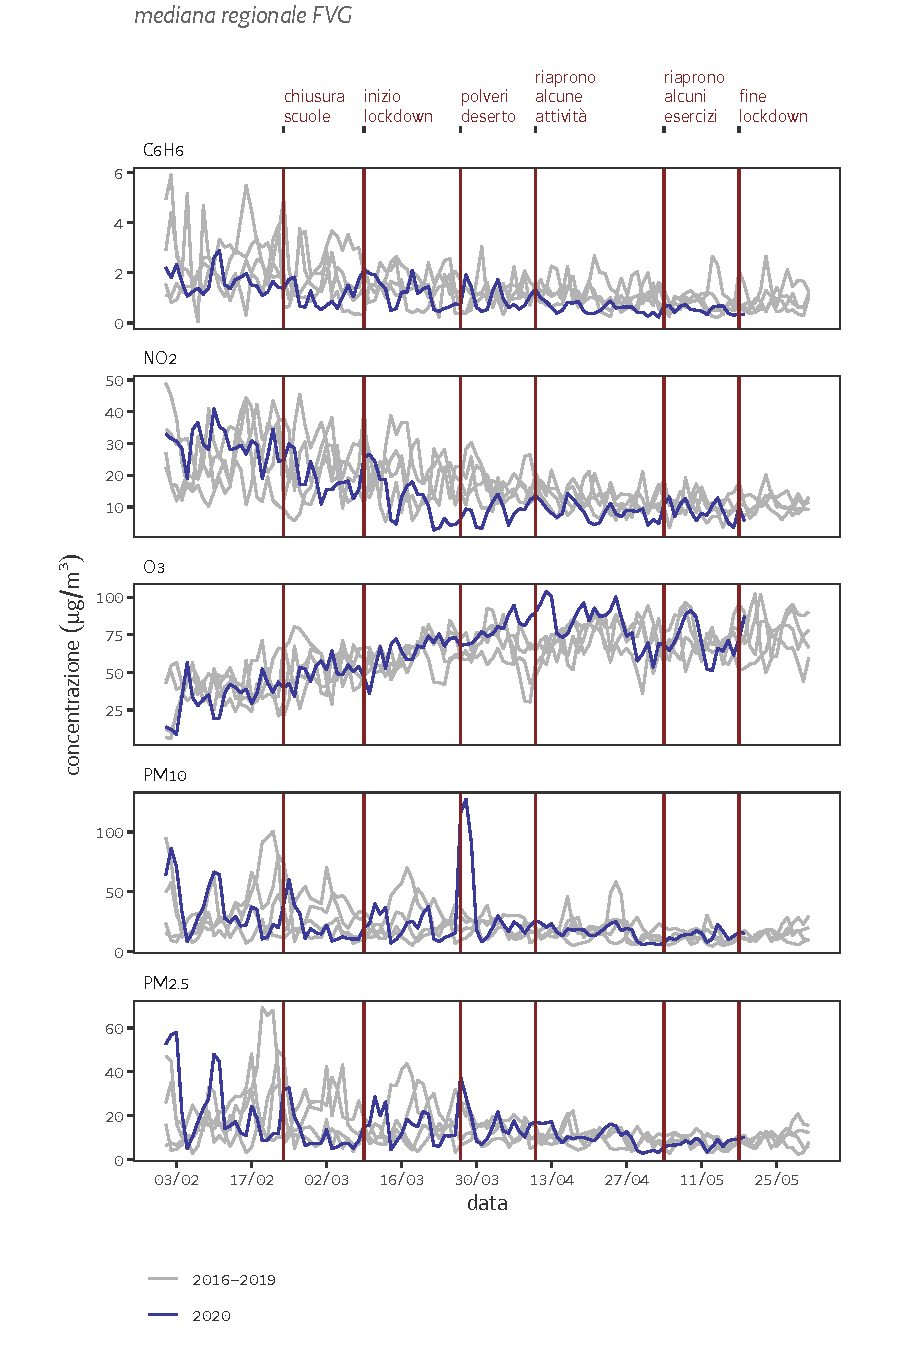
\includegraphics[trim=0 0 0 1cm, clip,width=0.85\textwidth]{{figs/dailyLastVsPast_20200201-20200531}.pdf}
    \caption[Andamento delle concentrazioni dei principali inquinanti, mediana regionale]{Andamento delle concentrazioni aria ambiente dei principali inquinanti, nel periodo febbraio--maggio 2020. Mediane giornaliere regionali in Friuli Venezia Giulia, confrontate con lo stesso periodo degli anni precedenti. Dall'alto: benzene, biossido di azoto, ozono, polveri sottili PM10 e PM2.5}
    \label{fig:andaminq}
\end{figure}

\begin{figure}
    \centering
    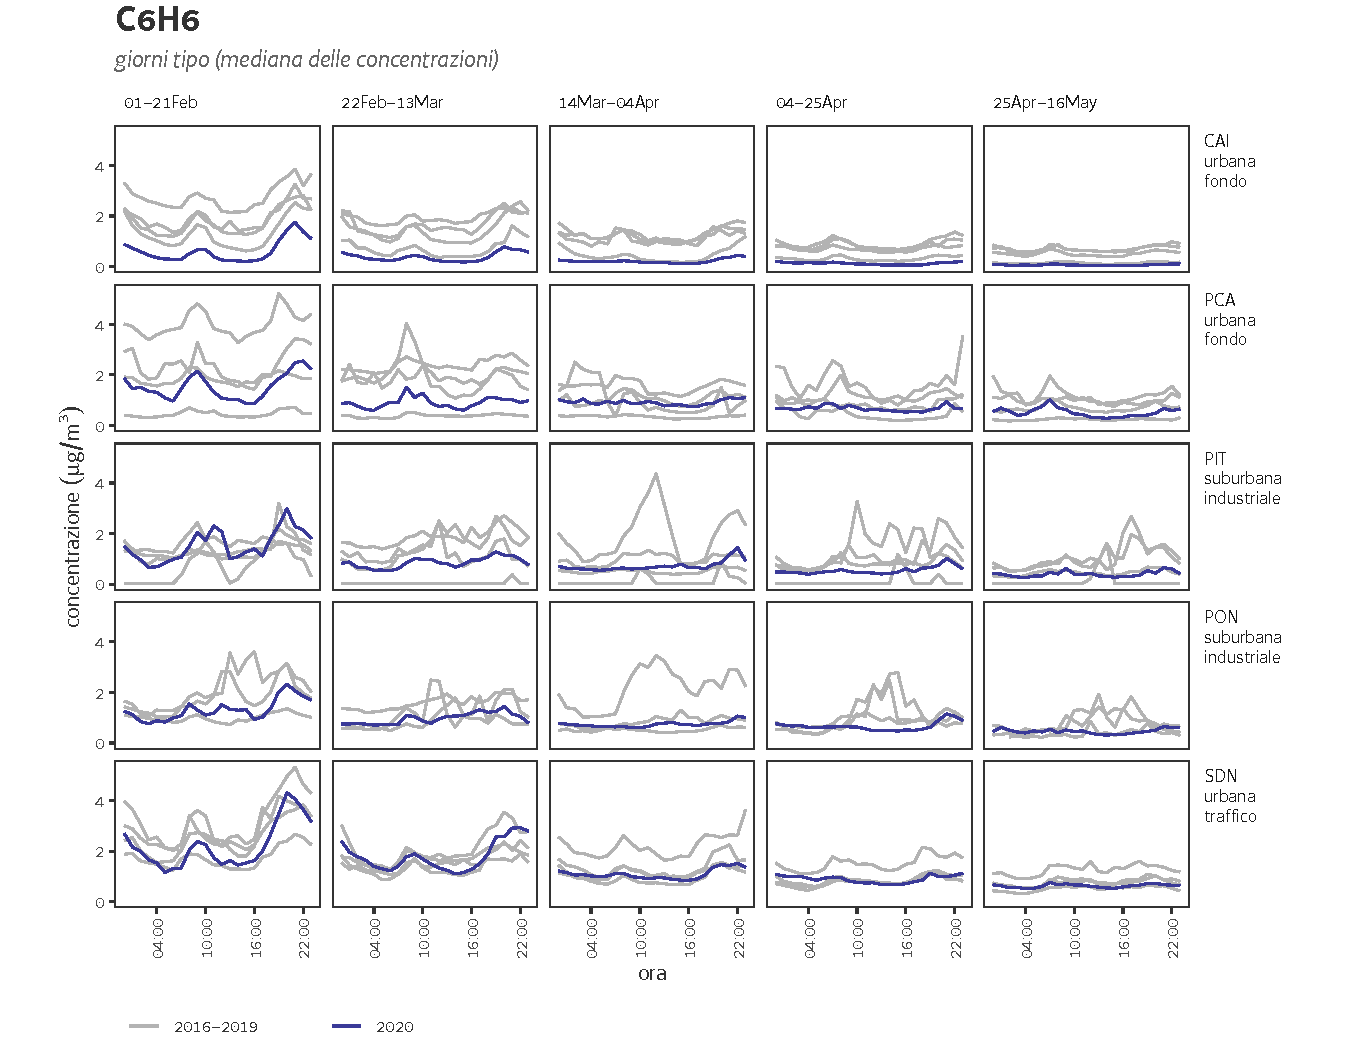
\includegraphics[width=\textwidth,page=1]{{figs/medianDay_LastVsPast_20200201-20200516}.pdf}
    \caption[Giorni tipo del benzene]{Giorni tipo delle concentrazioni di benzene calcolati ogni tre settimane nel periodo 1 febbraio -- 16 maggio 2020, confrontati con gli anni precedenti.}
    \label{fig:giornibenzene}
\end{figure}

\begin{figure}
    \centering
    \includegraphics[width=\textwidth,page=2]{{figs/medianDay_LastVsPast_20200201-20200516}.pdf}
    \caption[Giorni tipo del biossido di azoto]{Giorni tipo delle concentrazioni di biossido di azoto calcolati ogni tre settimane nel periodo 1 febbraio -- 16 maggio 2020, confrontati con gli anni precedenti.}
    \label{fig:giornino2}
\end{figure}

\begin{figure}
    \centering
    \includegraphics[width=\textwidth,page=3]{{figs/medianDay_LastVsPast_20200201-20200516}.pdf}
    \caption[Giorni tipo dell'ozono]{Giorni tipo delle concentrazioni di ozono calcolati ogni tre settimane nel periodo 1 febbraio -- 16 maggio 2020, confrontati con gli anni precedenti.}
    \label{fig:giornio3}
\end{figure}

\begin{figure}
    \centering
    \includegraphics[width=\textwidth,page=4]{{figs/medianDay_LastVsPast_20200201-20200516}.pdf}
    \caption[Giorni tipo del PM10]{Giorni tipo delle concentrazioni di polveri sottili PM10 calcolati ogni tre settimane nel periodo 1 febbraio -- 16 maggio 2020, confrontati con gli anni precedenti.}
    \label{fig:giornipm10}
\end{figure}
